\section{Degenerate Electron Gas, Part 1}
The office hours for this course will be Monday 4-5pm with Marcel, and 4-5pm on Tuesday with Oguzhan.

\subsection{Introducing the Degenerate Electron Gas}
\begin{figure}[htbp]
    \centering
    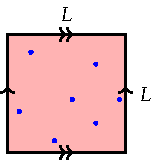
\includegraphics[]{Images/fig-jelliumcartoon.pdf}
    
    \caption{A cartoon depiction of the degenerate electron gas model. We consider a fixed, finite number of electrons $N$ in a three-dimensional box with side length $L$ and periodic boundary conditions. The electrons feel a uniformly distributed background of positive charge.}
    \label{fig-jelliumcartoon}
\end{figure}
Also known as the ``Jellium Model'', we consider a gas of electrons moving in a uniformly distributed background of positive charge. We begin with a 3d box of size $L$, and then take the thermodynamic limit of $L \to \infty$. 

We will use periodic boundary conditions, so if an electron leaves the box from one side, it comes in from the other. This is convenient as then the model admits plane waves solutions. We could use hard boundaries, and the description should agree in the $L \to \infty$ limit, but this set of boundary conditions is harder to work with; we would have cosine and and sines instead of plane waves.

The plane-wave basis will be a natural choice given the periodic BCs. Explicitly, we can write this as:
\begin{equation}
    \psi_{k, \lambda}(\v{x}) = \frac{1}{\sqrt{V}}e^{i\v{k} \cdot \v{x}}\eta_\lambda
\end{equation}
with $\lambda = (\uparrow, \downarrow)$ is the spin index. We have the spinors:
\begin{equation}
    \eta_\uparrow = \m{1\\0}, \quad \eta_\downarrow = \m{0\\1}
\end{equation}
The momentum is given by:
\begin{equation}
    \v{k} = (k_x, k_y, k_z), k_i = \frac{2\pi}{L}n_i
\end{equation}
where $n_i \in \ZZ$. The Hamiltonian is given by:
\begin{equation}
    \begin{split}
        H &= H_{el} + H_b + H_{el-b}
        \\ H_{el} &= \sum_{i=1}^N \frac{p_i^2}{2m} + \frac{1}{2}e^2\sum_{i \neq j} \frac{e^{-\mu\abs{\v{r}_i - \v{r}_j}}}{\abs{\v{r}_i - \v{r}_j}}
        \\ H_b &= \frac{1}{2}e^2 \int d^3x d^3x' \frac{n(\v{x})n(\v{x}')e^{-\mu\abs{\v{x} - \v{x}'}}}{\abs{\v{x} - \v{x}'}}
        \\ H_{el-b} &= -e\sum_{i=1}^N \int d^3x \frac{n(\v{x})e^{-\mu\abs{\v{x} - \v{r}_i}}}{\abs{\v{x} - \v{r}_i}}.
    \end{split}
\end{equation}
$H_{el}$ is just the kinetic energy of the electrons and the point-charge on point-charge interactions. $H_b$ is the electrostatic interaction of the background field with itself. And $H_{el-b}$ is the electrostatic interactions of the electrons with the background field. $N$ is the number of electrons, $V = L^3$ is the volume, $n = N/V$ is the electron density, and $\mu$ is a convergence factor which we send $\mu \to 0$\footnote{In nuclear physics this has significance as the \emph{Yukawa potential}; here we just use it as a convenient trick to remove some diverging integrals}. 

\subsection{Simplifying the background terms}
We want to rewrite this in second quantization notation. Only $H_e$ will have nontrivial structure in the second quantization notation, but nevertheless the other terms are necessary for the stability of the system.

Let us start with the second term, which is the simplest. We deal with a uniform background density, namely $n(\v{x}) = n = N/V$. $H_b$ then becomes a simple integral:
\begin{equation}
    \begin{split}
        H_b &= \frac{1}{2}e^2\left(\frac{N}{V}\right)^2 \int d^3x \int d^3 x' \frac{e^{-\mu\abs{\v{x} - \v{x}'}}}{\abs{\v{x} - \v{x}'}}.
        \\ &= \frac{1}{2}e^2\left(\frac{N}{V}\right)^2 \int d^3x \int d^3z \frac{e^{-\mu z}}{z}
        \\ &= \frac{1}{2}e^{2}\left(\frac{N^2}{V}\right)\frac{4\pi}{\mu^2}
    \end{split}
\end{equation}
Where in the second equality we use $z = \v{x}' - \v{x}$ in order to make the integrals independent, and evaluate the integrals in the third equality (the inner integral evaluating to $\frac{4\pi}{\mu^2}$, the outer to $V$). We can see why it was useful to introduce the $e^{-\mu}$; the integral would have diverged otherwise due to the long-range nature of the Coloumb interaction. Note also that we performed the integral assuming $\mu^{-1} \ll L$. We can similarly calculate $H_{el-b}$:
\begin{equation}
    \begin{split}
        H_{el-b} &= -e\frac{N}{V}\sum_{i=1}^N \int d^3x \frac{e^{-\mu\abs{\v{x} - \v{r}_i}}}{\abs{\v{x} - \v{r}_i}}
        \\ &= -e\frac{N}{V}\sum_{i=1}^N \int d^3z \frac{e^{-\mu z}}{z}
        \\ &= -e^2 \frac{N}{V} N \int d^3z\frac{e^{-\mu z}}{z}
        \\ &= -e^2\frac{N^2}{V}\frac{4\pi}{\mu^2}
    \end{split}
\end{equation}
We note the partial cancellation of the $H_b$ and the $H_{el-b}$ terms of the Hamiltonian; we will see another cancellation later.

A reasonable question is why the $\mu^{-1} \ll L$ assumption is necessary. It boils down to the the fact that we have periodic boundary conductions, and we do \emph{not} want the electric field of a given electron to interact with itself (or at least, not in a way that is exponentially insignificant and hence ignorable). See Fig. \ref{fig-jelliumlengthassumption} below for a visual demonstration of the importance of this assumption.

\begin{figure}[htbp]
    \centering
    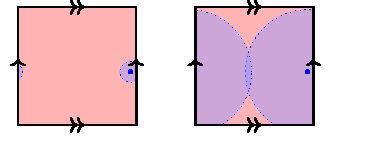
\includegraphics[]{Images/fig-jelliumlengthassumption.pdf}
    
    \caption{Comparisons of ``spheres of interaction'' of electrons when $\mu^{-1} \ll L$ (left) and $\mu^{-1} \sim L$ (right). We can see that in the former case, the electron does not interact with itself through the periodic boundary condition (beyond a negligeble exponentially small contribution), and so the system is physically sound. In the latter case, the electron does have a nontrivial interaction with its own electric field, as seen through the overlap of the sphere of interaction; this is not physical. Hence in our analysis of the Jellium model, we make the assumption that $\mu^{-1} \ll L$.}
    \label{fig-jelliumlengthassumption}
\end{figure}

With these simplifications, 
\begin{equation}
    H = -\frac{1}{2}e^2\frac{N^2}{V}\frac{4\pi}{\mu^2} + H_{el}
\end{equation}
Note that all of the interesting physics is contained in $H_{el}$, but we need $H_b + H_{el}$ to get a finite theory; we can see that if we took $\mu \to 0$ now, the energy would diverge; presumably there will be some sort of cancellation that occurs with $H_{el}$ that will regularize the theory. 

\subsection{Second Quantization of the Electron Term}
Let us now transform the $H_{el}$ term into second quantized notation.
\begin{enumerate}[(i)]
    \item We start with the kinetic energy term:
    \begin{equation}
        \begin{split}
            \bra{\v{k}_1\lambda_1}T\ket{\v{k}_2\lambda_2} &= \frac{1}{2mV}\int d^3x e^{-i\v{k} \cdot \v{x}}\eta_{\lambda_1}^\dag (-\hbar^2\nabla^2)e^{i\v{k}_2\cdot \v{x}}\eta_{\lambda_2}
            \\ &= \frac{\hbar^2 k_2^2}{2mV}\delta_{\lambda_1\lambda_2}\int d^3x e^{-i\v{x} \cdot (\v{k}_1 - \v{k_2})}
            \\ &= \frac{\hbar^2k_2^2}{2m}\delta_{\lambda_1\lambda_2}\delta_{\v{k}_1\v{k}_2}
        \end{split}
    \end{equation}
    where we use that $\int d^3x e^{-i\v{x} \cdot (\v{k}_1 - \v{k_2})} = V\delta_{k_1k_2}$. Wee therefore obtain:
    \begin{equation}
        \hat{T} = \sum_{k, \lambda}\frac{\hbar^2 k^2}{2m}c_{k\lambda}^\dag c_{k\lambda}.
    \end{equation}
    \item We now look at the potential term:
    \begin{equation}
        \bra{k_1\lambda_1k_2\lambda_2}V\ket{k_3\lambda_3k_4\lambda_4} = \frac{e^2}{V}\delta_{\lambda_1\lambda_3}\delta_{\lambda_2\lambda_4}\delta_{k_1 + k_2, k_3 + k_4}\frac{4\pi}{(\v{k}_1 - \v{k}_3)^2 + \mu}.
    \end{equation}
    See F\&W for details; there is nothing conceptually new in the calculation above, it is only slightly more annoying at there are four plane wave terms.
\end{enumerate}
We therefore obtain:
\begin{equation}\label{eq-JelliumquantizedH}
    \hat{H} = \hat{T} - \frac{1}{2}\frac{e^2N^2}{V}\frac{4\pi}{\mu} + \frac{e^2}{2V}\sum_{k, \lambda}\delta_{\lambda_1\lambda_3}\delta_{\lambda_2\lambda_4}\delta_{k_1 + k_2, k_3 + k_4}\frac{4\pi}{(\v{k}_1 - \v{k}_3)^2 + \mu} c^\dag_{k_1\lambda_1}c^\dag_{k_2\lambda_2}c_{k_4\lambda_4}c_{k_3\lambda_3}.
\end{equation}
Now we have to think a little bit; we have three delta functions, two for spin, one for momenta. We can explicitly two summations over $\lambda$ and one over momentum. Instead of doing so blindly, we will find it useful to make the following change of variables:
\begin{equation}
    \m{\v{k}_1 = \v{k} + \v{q} & \v{k}_3 = \v{k} \\ \v{k}_2 = \v{p} - \v{q} & \v{k}_4 = \v{p}} \quad \m{\lambda_1 = \alpha \\ \lambda_2 = \beta}
\end{equation}
We may notice that we express the four momenta in terms of three, but this is ok; we have the extra constraint on the momentum already, and it was designed to satisfy this constraint. Substituting, the potential term becomes:
\begin{equation}
    \frac{e^2}{2V}\sum_{\v{k}\v{p}\v{q}}\sum_{\alpha\beta}\frac{4\pi}{\v{q}^2 + \mu^2}c^\dag_{\v{k} + \v{q}\alpha}c^{\dag}_{\v{p} - \v{q}\beta}c_{\v{p}\beta}c_{\v{k}\alpha}.
\end{equation}
We now want to send $\mu \to 0$. Note that we can do this for any term in the sum for which $\v{q} \neq \v{0}$. The only singular term is $\v{q} = \v{0}$, so let us study that term:
\begin{equation}\label{eq-badtermJellium}
    \begin{split}
        \frac{e^2}{2V}\sum_{\v{k}\v{p}}\sum_{\alpha\beta}\frac{4\pi}{\mu^2}c^\dag_{\v{k}\alpha}c^{\dag}_{\v{p}\beta}c_{\v{p}\beta}c_{\v{k}\alpha} &= \frac{e^2}{2V}\sum_{\v{k}\v{p}}\sum_{\alpha\beta}\frac{4\pi}{\mu^2}c^\dag_{\v{k}\alpha}(c_{\v{k}\alpha}c^\dag_{\v{p}\beta} - \delta_{\v{k}\v{p}}\delta_{\alpha\beta})c_{\v{p}\beta}
        \\ &= \frac{e^2}{2V}\frac{4\pi}{\mu^2}(\hat{N}^2 - \hat{N})
        \\ &=\frac{e^2}{2}\frac{N^2}{V}\frac{4\pi}{\mu^2} - \frac{e^2}{2}\frac{N}{V}\frac{4\pi}{\mu^2}
    \end{split}
\end{equation}
where in the first equality we have commuted the $c_{\v{k}\alpha}$ between the two $c^\dag$s (being careful to respect the commutation relations), in the second equality we have used the definition of the number operator, and in the third equality we used the fact that we work with a system with a finite, fixed number of electrons and hence we can replace the operators $\hat{N}$ with the number of particles $N$. 

We see that the first term in Eq. \eqref{eq-badtermJellium} and the second term in Eq. \eqref{eq-JelliumquantizedH} cancel. We argue that the second term in Eq. \eqref{eq-badtermJellium} is vanishingly small in the thermodynamic limit. We argue this as follows; since $N/V$ (the number density) is constant with the system size, the term is constant with the system size; however $\avg{H}$ is extensive, and scales with the system size ($\avg{H} \sim V \sim N$). Hence we may choose to ignore it. So let us conclude by stating our final Hamiltonian:
\begin{equation}
    \hat{H} = \sum_{k\alpha}\frac{\hbar^2k^2}{2m}c^\dag_{k\lambda}c_{k\lambda} + \frac{e^2}{2V}\sum_{\v{k}\v{p}\v{q}}'\sum_{\alpha\beta} \frac{4\pi}{\v{q}^2}c^\dag_{\v{k} + \v{q}\alpha}c^{\dag}_{\v{p} - \v{q}\beta}c_{\v{p}\beta}c_{\v{k}\alpha}
\end{equation}
where the prime on the summation denotes that we do not include the $\v{q} = 0$ term.